\documentclass{sig-alternate}

\usepackage{bm}
\usepackage{bbm}
\usepackage{amsmath}
\usepackage{alltt, amssymb,stmaryrd}
\usepackage{color}
\usepackage{mdwlist}
\usepackage{float}
\usepackage{hyperref}

\usepackage{algorithm}
\usepackage{algorithmic}
\renewcommand{\algorithmicrequire}{\textbf{Input:}}
\renewcommand{\algorithmicensure}{\textbf{Output:}}

\def\C {\ensuremath{\mathsf{C}}}
\def\M {\ensuremath{\mathsf{M}}}
\def\Q {\ensuremath{\mathbb{Q}}}
\def\N {\ensuremath{\mathbb{N}}}
\def\R {\ensuremath{\mathbb{R}}}
\def\Z {\ensuremath{\mathbb{Z}}}
\def\F {\ensuremath{\mathbb{F}}}
\def\H {\ensuremath{\mathbb{H}}}
\def\K {\ensuremath{\mathbb{K}}}
\def\Kbar {\ensuremath{\overline{\mathbb{K}}}}
\def\L {\ensuremath{\mathbb{L}}}
\def\A {\ensuremath{\mathbb{A}}}
\def\B {\ensuremath{\mathbb{B}}}

\def\va {\ensuremath{\mathsf{a}}}
\def\vy {\ensuremath{\mathsf{a}}}
\def\vu {\ensuremath{\mathsf{u}}}
\def\vb {\ensuremath{\mathsf{b}}}
\def\vc {\ensuremath{\mathsf{c}}}

\def\mul {\ensuremath{\mathsf{mul}}}
\def\rem {\ensuremath{\mathsf{rem}}}
\def\cat {\ensuremath{\mathsf{cat}}}
\def\coeff {\ensuremath{\mathsf{coefficient}}}
\def\mulmod {\ensuremath{\mathsf{mulmod}}}
\def\rev {\ensuremath{\mathsf{rev}}}
\def\x {\ensuremath{\mathbf{x}}}
\def\Tr {\ensuremath{\mathrm{Tr}}}
\DeclareBoldMathCommand{\bxi}{\xi}
\DeclareBoldMathCommand{\bupsilon}{\upsilon}
\DeclareBoldMathCommand{\bzeta}{\zeta}
\DeclareBoldMathCommand{\blambda}{\lambda}

\newcounter{algo}

\newenvironment{algorithm_noendline}[4]{\small\begin{center}\begin{minipage}{0.48\textwidth}
      \refstepcounter{algo}
      \label{#4}
      \sf
      \rule{\textwidth}{0.2pt}\\
      \makebox[\textwidth][c]{Algorithm~\arabic{algo}:~\textbf{#1}}\\
      \rule[0.5\baselineskip]{\textwidth}{0.2pt}\\

      \vspace{-12pt}

      \parbox{\textwidth}{\textbf{Input} #2}
      \parbox{\textwidth}{\textbf{Output} #3}

\vspace{-7pt}

      \begin{enumerate*}}{\end{enumerate*}
      \vspace{-11pt}
\end{minipage}\end{center}
}

\newenvironment{algorithm_endline}[4]{\small\begin{center}\begin{minipage}{0.48\textwidth}
      \refstepcounter{algo}
      \label{#4}
      \sf
      \rule{\textwidth}{0.2pt}\\
      \makebox[\textwidth][c]{Algorithm~\arabic{algo}:~\textbf{#1}}\\
      \rule[0.5\baselineskip]{\textwidth}{0.2pt}\\

      \vspace{-12pt}

      \parbox{\textwidth}{\textbf{Input} #2}
      \parbox{\textwidth}{\textbf{Output} #3}

\vspace{-7pt}

      \begin{enumerate*}}{\end{enumerate*}
      \vspace{-11pt}
      \rule{\textwidth}{0.2pt}
\end{minipage}\end{center}
%\vspace{-0.5cm}
}

\floatstyle{plain}
\newfloat{algofloat}{thp}{bla}
\floatname{algofloat}{}

\newcommand{\wrt}{\vdash} 
\newcommand{\ang}[1]{\langle#1\rangle}
\newcommand{\dual}[1]{\overline{#1}}
\newcommand{\todo}[1]{\textcolor{red}{TODO: #1}}

\def\gathen#1{{#1}}
\def\hoeven#1{{#1}}

\newtheorem{Def}{Definition}
\newtheorem{Theo}{Theorem}
\newtheorem{Prop}{Proposition}
\newtheorem{Lemma}{Lemma}

\numberofauthors{3}
\author{
  \alignauthor Luca De Feo\\
  \affaddr{Laboratoire PRiSM}\\
  \affaddr{Universit\'e de Versailles}\\
  \email{luca.de-feo@uvsq.fr}
  \alignauthor Javad Doliskani\\
  \affaddr{Computer Science Department}\\
  \affaddr{Western University}\\
  \email{jdoliska@uwo.ca}
  \alignauthor \'Eric Schost\\
  \affaddr{Computer Science Department}\\
  \affaddr{Western University}\\
  \email{eschost@uwo.ca}
}

\title{Fast arithmetic for the algebraic closure of finite fields}

\begin{document}

\maketitle
\begin{abstract}
  We present algorithms to construct and do arithmetic operations in
  the algebraic closure of the finite field $\mathbb{F}_p$. Our
  approach is inspired by algorithms for constructing irreducible
  polynomials, which first reduce to prime power degrees, then use
  composita techniques. We use similar ideas to give efficient
  algorithms for embeddings and isomorphisms.
\end{abstract}

\category{F.2.1}{Theory of computation}{Analysis of algorithms and problem complexity}[Computations in finite fields]
\category{G.4}{Mathematics of computing}{Mathematical software}
\terms{Algorithms,Theory}
\keywords{Finite fields, irreducible polynomials, extensions.}

%%%%%%%%%%%%%%%%%%%%%%%%%%%%%%%%%%%%%%%%%%%%%%%%%%%%%%%%%%%%
%%%%%%%%%%%%%%%%%%%%%%%%%%%%%%%%%%%%%%%%%%%%%%%%%%%%%%%%%%%%
%%%%%%%%%%%%%%%%%%%%%%%%%%%%%%%%%%%%%%%%%%%%%%%%%%%%%%%%%%%%

\section{Introduction}

Several computer algebra systems or libraries, such as
Magma~\cite{MAGMA}, Sage~\cite{Sage}, NTL~\cite{shoup2003ntl} or
Flint~\cite{hart2010flint}, offer built-in features to build and
compute in arbitrary finite fields. At the core of these designs, one
finds algorithms for building irreducible polynomials and algorithms
to compute embeddings and isomorphisms. The
paper~\cite{bosma+cannon+steel97} describes the system used in Magma,
one of the most complete we are aware of.

Previous algorithms typically rely on linear algebra techniques, for
instance to describe embeddings or isomorphisms (this is the case for
the algorithms in~\cite{bosma+cannon+steel97}, but also for those
in~\cite{LenstraJr91,Allombert02}). Unfortunately, linear algebra
techniques have cost at least quadratic in the degree of the
extensions we consider, and (usually) quadratic memory requirements.
Our goal here is to replace linear algebra by polynomial arithmetic,
exploiting fast polynomial multiplication to obtain algorithms of
quasi-linear complexity. As we will see, we meet this goal for
several, but not all, operations.

\paragraph*{{\bf \rm Setup}}
Let $p$ be a prime (that will be fixed throughout this paper). We are
interested in describing extensions $\F_{p^n}$ of $\F_p$; such an
extension has dimension $n$ over $\F_p$, so representing an element in
it involves $n$ base field elements.

It is customary to use polynomial arithmetic to describe these
extensions (but not necessary: Lenstra's algorithm~\cite{LenstraJr91}
uses an entire multiplication tensor, which has size $n^3$). Given an
extension degree $n$, a first step is then to construct an irreducible
polynomial $Q_n$ of degree $n$ in $\F_p[x]$. This will allow us to
identify $\F_{p^n}$ with $\F_p[x]/\ang{Q_n}$; then, using fast
Euclidean division and extended GCD, operations $(+,\times,\div)$ in
$\F_p[x]/\ang{Q_n}$ all take quasi-linear time in~$n$.

However, this is not sufficient, as we also want mechanisms to perform
(for instance) field embeddings. Given irreducible polynomials $Q_m$
and $Q_n$ over $\F_p$, with $\deg(Q_m)=m$ dividing $\deg(Q_n)=n$,
there certainly exist algorithms that determine an embedding
$\F_p[x]/\ang{Q_m} \to \F_p[x]/\ang{Q_n}$. However, as said above,
most algorithms use linear algebra techniques. In order for the system
to be consistent, note that these embeddings must be {\em
  compatible}~\cite{bosma+cannon+steel97}.

To bypass these issues, we use an approach inspired by e.g. Shoup's
algorithm for computing irreducible polynomials~\cite{Shoup90,shoup94}
(see also~\cite{couveignes+lercier11,lenstra+desmit08-stdmodels}):
first reduce to the case of prime power degrees, then use composita
techniques, in a manner that ensures compatibility of the embeddings
automatically.

\smallskip\noindent{{\bf \rm Background: towers.}}
Suppose that for any prime $\ell$, an {\em $\ell$-adic tower} over
$\F_p$ is available. By this, we mean a family of polynomials
$(T_{\ell,i})_{i \ge 1}$, with $T_{\ell,i} \in \F_p[x_1,\dots,x_i]$,
monic of degree $\ell$ in $x_i$, such that for all $i$ the ideal
$\ang{T_{\ell,1},\dots,T_{\ell,i}}$ is prime in $\F_p[x_1,\dots,x_i]$.
Our model of the field with $p^{\ell^i}$ elements could then
be
$\K_{\ell^i}=\F_p[x_1,\dots,x_i]/\ang{T_{\ell,1},\dots,T_{\ell,i}}$,
but we prefer to work with univariate polynomials (the cost of
arithmetic operations is higher in the multivariate basis).  

For $1 \le i \le n$, let then $Q_{\ell,i}$ be the minimal polynomial
of $x_i$ in the extension $\F_p \to \K_{\ell^n}$. This polynomial does
not depend on $n$, but only on $i$; it is monic, irreducible of degree
$\ell^i$ in $\F_p[x_i]$ and allows us to define $\F_{p^{\ell^i}}$ as
$\F_p[x_i]/\ang{Q_{\ell,i}}$.
For $1 \le i \le j \le n$, let further $Q_{\ell,i,j-i}$ be the minimal
polynomial of $x_j$ in the extension $\F_p[x_i]/\ang{Q_{\ell,i}} \to
\K_{\ell^n}$ (as above, it does not depend on $n$). This polynomial is
monic, irreducible of degree $\ell^{j-i}$ in
$\F_{p^{\ell^i}}[x_j]=\F_p[x_i]/\ang{Q_{\ell,i}}[x_j]$.

Thus, $\F_p[x_j]/\ang{Q_{\ell,j}}$ and
$\F_p[x_i,x_j]/\ang{Q_{\ell,i},Q_{\ell,i,j-i}}$ are two models for
$\F_{p^{\ell^j}}$. Provided conversion algorithms between these
representations are available, we can perform embeddings (that will
necessarily be compatible) between different levels of the $\ell$-adic
tower, \emph{i.e.}\ extensions of degrees $(\ell^i)_{i \ge 1}$.

Such towers, together with efficient conversion algorithms, were
constructed in the cases $\ell = p$
in~\cite{cantor89,couveignes00,df+schost12}, $\ell=2$
in~\cite{DoSc12}, and for other values of $\ell$ in~\cite{DeDoSc13}.
Thus, it remains to give algorithms to ``glue'' towers defined for
different values of $\ell$. This is the purpose of this paper.

\smallskip\noindent{{\bf \rm Our contribution.}} The algorithms used
in the constructions of the towers are inspired by those used
in~\cite{Shoup90,shoup94,couveignes+lercier11} to construct
irreducible polynomials. Also used in these references is the
following idea: let $Q_m(x)$ and $Q_n(y)$ be irreducible polynomials
over $\F_p$, with coprime degrees $m$ and $n$, and having respectively
$(a_i)_{1 \le i \le m}$ and $(b_j)_{1 \le j \le n}$ as roots in an
algebraic closure of $\F_p$. Then their {\em composed product}
$Q_{mn} = \prod_{1 \le i \le m, 1 \le j \le n} (z- a_i b_j)$ is
irreducible of degree $mn$ in $\F_p[z]$

In this paper, we use an {\em algebraic complexity model}, where the
cost of an algorithm is counted in terms of the number of operations
$(+,\times,\div)$ in $\F_p$.  If the goal is building irreducible
polynomials, then computing $Q_{mn}$ is enough: an algorithm given
in~\cite{BoFlSaSc06} has quasi-linear cost in $mn$. Our goal here is
to give algorithms for further operations: computing embeddings of the
form $\varphi_x: \F_p[x]/\ang{Q_m}\to \F_p[z]/\ang{Q_{mn}}$ or
$\varphi_y: \F_p[y]/\ang{Q_n}\to \F_p[z]/\ang{Q_{mn}}$, and the
isomorphism $\Phi: \F_p[x,y]/\ang{Q_m,Q_n}\to \F_p[z]/\ang{Q_{mn}}$ or
its inverse.

Standard solutions to these questions exist, using {\em modular
  composition} techniques: once the image $S=\Phi(x)$ is known,
computing $\varphi_x(a)$ amounts to computing $a(S) \bmod Q_{mn}$;
similarly, computing $\Phi(b)$, for $b$ in $\F_p[x,y]/\ang{Q_m,Q_n}$,
amounts to computing $b(S,T) \bmod Q_{mn}$, with $T=\Phi(y)$.  This
can be done using the Brent and Kung algorithm~\cite{brent+kung}: the
resulting cost is $O(m n^{(\omega+1)/2}) \subset O(m n^{1.69})$ for
$\varphi_x$ (see the analysis in~\cite{shoup94}) and $O((m
n)^{(\omega+1)/2}) \subset O(m^{1.69} n^{1.69})$ for $\Phi$ or its
inverse~\cite{PoSc13b}. Here, we denote by $\omega$ a constant in
$(2,3]$ such that one can multiply matrices of size $m$ over any ring
  $A$ using $O(m^\omega)$ operations $(+,\times)$ in~$A$; using the
  algorithms of~\cite{coppersmith+winograd,Williams12}, we can take
  $\omega \le 2.38$.

Our main result improves on these former ones. We denote by $\M:\N \to
\N$ a function such that for any ring $A$, polynomials in $A[x]$ of
degree at most $n$ can be multiplied in $\M(n)$ operations
$(+,\times)$ in $A$, and we make the usual super-linearity assumptions
on $\M$~\cite[Chapter~8]{vzGG}.
\begin{Theo}\label{theo:main}
  One can apply $\varphi_x$ (resp.\ $\varphi_y$) to an element of
  $\F_p[x]/\ang{Q_m}$ (resp.\ $\F_p[x]/\ang{Q_n}$), or invert it on its
  image, using $O(n\M(m)+m\M(n))$ operations in $\F_p$.

  Suppose without loss of generality that $m \le n$. Then one can
  apply $\Phi$ to an element of $\F_p[x,y]/\ang{Q_m, Q_n}$, or invert it, using either
  $O(m^2 \M(n))$ or $O(\M(mn)n^{1/2}+\M(m) n^{(\omega+1)/2} )$
  operations in $\F_p$.
\end{Theo}

Using the $O\tilde{~}$ notation to neglect polylogarithmic factors, we
can take $\M(n) \in O\tilde{~}(n)$.  Then, our algorithm for
embeddings and their inverses has quasi-linear complexity
$O\tilde{~}(mn)$. Our two solutions for $\Phi$ or its inverse have
respective costs $O\tilde{~}(m^2 n)$ and $O\tilde{~}(m
n^{(\omega+1)/2})$. The minimum of the two is seen to lie in
$O\tilde{~}( (mn)^{2\omega/(\omega+1)})$; for $\omega \in (2,3]$, the
resulting exponent lies in $(1.333\dots, 1.5]$.  Thus, although our
algorithm for embedding is essentially optimal, our algorithm for
isomorphism is not (but it improves on previous results).

We point out that if $S=\Phi(x)$ and $T=\Phi(y)$ are known, a result
by Kedlaya and Umans~\cite{KeUm11} for modular composition, and its
extension in~\cite{PoSc13a}, yield an algorithm with {\em boolean
  complexity} essentially linear in $mn$ and $\log(p)$ (on a
RAM). Unfortunately, these algorithms seem to be unfeasible for the
moment, indeed we are not aware of any implementation. It is also
worth noting that our algorithms apply in a more general setting than
finite fields (mild assumptions are required).

\noindent{\bf Outline.}  Section~\ref{sec:prelim} presents basic
algorithms for polynomials, as well as their {\em transposes}.  In
Sections~\ref{sec:trace}, we introduce the main idea behind our
algorithms: the trace induces a natural duality on algebras of the
form $\F_p[x]/\ang{Q}$, and some conversion algorithms will turn out
to be straightforward once expressed in dual bases; the algorithms are
detailed in Section~\ref{sec:emb-iso}. Section~\ref{sec:fpbar}
explains how the results in this paper can be used in order to
construct the algebraic closure of $\F_p$, and we conclude with some
experimental results.

%%%%%%%%%%%%%%%%%%%%%%%%%%%%%%%%%%%%%%%%%%%%%%%%%%%%%%%%%%%%
%%%%%%%%%%%%%%%%%%%%%%%%%%%%%%%%%%%%%%%%%%%%%%%%%%%%%%%%%%%%
%%%%%%%%%%%%%%%%%%%%%%%%%%%%%%%%%%%%%%%%%%%%%%%%%%%%%%%%%%%%

\section{Preliminaries}\label{sec:prelim}

We recall first previous results concerning polynomial arithmetic and
transposition of algorithms. In all this section, a ground field $k$,
non necessarily finite, is fixed. For integers $m,n$, we denote by
$k[x]_m$ (resp.\ $k[x,y]_{m,n}$) the set of polynomials $P$ in $k[x]$
with $\deg(P) <m$ (resp.\ $P$ in $k[x,y]$ with $\deg(P,x) <m$ and
$\deg(P,y)<n$).

%%%%%%%%%%%%%%%%%%%%%%%%%%%%%%%%%%%%%%%%%%%%%%%%%%%%%%%%%%%%

\subsection{Polynomial multiplication and remainder}

We start with some classical algorithms and their complexity; for all
the algorithms that follow, all polynomials are written on the
canonical monomial basis (this is innocuous for the moment, but other
bases will be discussed below).

The product of two polynomials of respective degrees at most $m$ and
$n$ can be computed in $\M(\max(m,n))$ operations in $k$.  If $P$ is a
monic polynomial of degree $m$ in $k[x]$, for $n \ge 1$, we let
$\rem(.,P,n)$ be the operator
$$
\begin{array}{cccc}
\rem(.,P,n): &k[x]_n& \to &k[x]_{m}\\
& a & \mapsto & a \bmod P.
\end{array}$$ 
For $n \le m$, this is free of cost. For $n > m$, this can be computed
in time $O(n\M(m)/m)$ using the Cook-Sieveking-Kung algorithm and
blocking techniques~\cite[Ch.~5.1.3]{Bostan10}. Defining
$A=k[x]/\ang{P}$, and choosing a fixed $b \in A$, we can then define
the mapping $\mulmod(.,b,P)$, which maps $a \in A$ to $ab \bmod P$; it
can be computed in time $O(\M(m))$. Finally, given an integer $m$, the
reversal operator in length $m$ is 
$$
\begin{array}{cccc}
\rev(.,m): &k[x]_m &\to& k[x]_m  \\
& a & \mapsto & x^{m-1} a(1/x).
\end{array}$$ 

%%%%%%%%%%%%%%%%%%%%%%%%%%%%%%%%%%%%%%%%%%%%%%%%%%%%%%%%%%%%

\subsection{The transposition principle}
\label{sec:algor-dual-basis}

The {\em transposition principle} is an algorithmic result which
states that given an algorithm that performs an $r \times s$
matrix-vector product $u \mapsto M u$, one can deduce an algorithm
with the same cost, up to $O(\max(r,s))$, which performs the
transposed matrix-vector product $v \mapsto M^t
v$~\cite[Ch.~13]{burgisser+clausen-shokrollahi}.

Although that theorem is constructive, the proof involves going down
to the DAG representation of the algorithm, which is hardly
convenient.  In the rest of this article, we will reuse techniques
from~\cite{bostan+lecerf+schost:tellegen} in order to simplify the
transposition process: in a nutshell, most of our algorithms will rely
on a few basic operations (such as polynomial or matrix
multiplication), and their transposes are obtained by transposing each
basic subroutine, and reversing their order.

Let us briefly review the transposes of operations described in the
previous subsection. The transpose of polynomial multiplication is
described in~\cite{bostan+lecerf+schost:tellegen}; it is closely
related to the {\em middle product}~\cite{hanrot+quercia+zimmermann}.
Let next $P$ be monic of degree $m$, and define
$A=k[x]/\ang{P}$. Denote by $A^\ast$ the dual space of $A$, i.e.\ the
$k$-linear forms on $A$, then we can then discuss the transposes of
$\rem$ and $\mulmod$. As shown
in~\cite{bostan+lecerf+schost:tellegen}, the dual map
$$
\begin{array}{cccc}
\rem^t(.,P,n): &k^m& \to &k^n
\end{array}$$ 
takes as input a form $\ell\in A^\ast$ given by the values
$(\ell(x^i))_{0 \le i < m}$; the output is then the values
$(\ell(x^i))_{0 \le i < n}$. For $n < m$, there is nothing to do. For
greater values of $n$, $\rem^t$ is \emph{linear sequence extension}:
it takes as input the initial $m$ values of a linear recurring
sequence of minimal polynomial $P$, and outputs its first $n$ values.
LFSRs give a simple, though suboptimal, implementation of this
operator. The transposed version of the Cook-Sieveking-Kung fast
Euclidean division algorithm yield better algorithms: like the
forward direction, the cost of the transposed algorithm is
$O(n\M(m)/m)$ operations in $k$~\cite{vzgathen+shoup92:journal,shoup99}.

Multiplication by a fixed $b\in A$ is a linear map $M_b:A\to A$. By
definition, the dual map $M_b^t: A^* \to A^*$ maps a linear form to $b
\cdot \ell$, which is such that $(b \cdot \ell)(a)
=\ell(ab)$. Algorithms for $\mulmod^t$ have been subject to much
research (for instance, Berlekamp's \emph{bit serial
  multiplication}~\cite{Berlekamp82} is a popular arithmetic circuit
for $\mulmod^t$ in the case $k=\F_2$); algorithms of cost $O(\M(m))$
are given in~\cite{shoup99,bostan+lecerf+schost:tellegen}. 

Lastly, the reversal operator on $k[x]_m$ is its own transpose.

%%%%%%%%%%%%%%%%%%%%%%%%%%%%%%%%%%%%%%%%%%%%%%%%%%%%%%%%%%%%
%%%%%%%%%%%%%%%%%%%%%%%%%%%%%%%%%%%%%%%%%%%%%%%%%%%%%%%%%%%%
%%%%%%%%%%%%%%%%%%%%%%%%%%%%%%%%%%%%%%%%%%%%%%%%%%%%%%%%%%%%

\section{Trace and duality}\label{sec:trace}

Next, we discuss some classical facts about dualities induced by
non-degenerate bilinear forms, pairs of primal / dual bases, and give
change-of-basis algorithms for a useful particular case. In all this
section, $k$ is a perfect field.

%%%%%%%%%%%%%%%%%%%%%%%%%%%%%%%%%%%%%%%%%%%%%%%%%%%%%%%%%%%%

\subsection{Duality}\label{ssec:duality}

A general reference for what follows
is~\cite[Ch.~IX.1.8]{BourbakiAlgCom9}. Let $E$ and $F$ be $k$-vector
spaces, with $\dim(E)=\dim(F) < \infty$; suppose further that
$\ang{.,.}: E\times F \to k$ is a non-degenerate bilinear form.
Then, to any vector space basis $\bxi=(\xi_i)_i$ of $E$, we
can associate a unique \emph{dual basis}
$\bxi^\ast=(\xi_i^\ast)_i$ of $F$ such that $
\ang{\xi_i,\xi^\ast_j} = \delta_{i,j}$ (the Kronecker symbol).

In other words, given $a$ in $F$, the coefficients $(a_i)$ of $a$ on
the basis $\bxi^\ast$ are given by $a_i=\ang{\xi_i, a}$. A
standard example (implicitly used in the previous section) is the case
where $F$ is the dual $E^*$ of $E$, with $\ang{v,\ell}=\ell(v)$ for
all $v\in E$ and $\ell \in E^*$; we will see in the next subsection
another family of examples, with $E=F$.

Let $E',F'$ be two further vector spaces, with $\dim(E')=\dim(F')$ and
let $\ang{.,.}'$ be a bilinear form $E'\times F' \to k$. Then, to
any linear mapping $u:E\to E'$, one associates its {\em dual}
(with respect to $\ang{.,.}$ and $\ang{.,.}'$), which is a linear
mapping $u^t: F' \to F$ characterized by the equality
$\ang{u(a),b'}'=\ang{a,u^t(b')}$, for all $a\in E$ and $b'$ in $F'$.

Let as above $\bxi$ be a basis of $E$, and let $\bxi^\ast$ be
the dual basis of $F$; consider as well a basis $\bupsilon$ of $E'$ and
its dual basis $\bupsilon^\ast$ of $F'$. If $M$ is the matrix of $u$ in
the bases $(\bxi,\bupsilon)$, the matrix of $u^t$ in the bases
$(\bupsilon^\ast,\bxi^\ast)$ is the transpose of $M$. The
transposition principle then implies that, from an algorithm that
computes $u: E \to E'$ in the bases $(\bxi,\bupsilon)$, we deduce the
existence of an algorithm for the dual map $u^t: F' \to F$ in the
bases $(\bupsilon^\ast,\bxi^\ast)$, with essentially the same cost.

%%%%%%%%%%%%%%%%%%%%%%%%%%%%%%%%%%%%%%%%%%%%%%%%%%%%%%%%%%%%

\subsection{Traces in reduced algebras}

General reference for the following
are~\cite{Kunz86,Cox-Little-OShea:UAG2005}. Suppose now that $s$ is a
positive integer, and $I$ a zero dimensional radical ideal in
$k[x_1,\dots,x_s]$. Thus, $A=k[x_1,\dots,x_s]/I$ is a reduced
$k$-algebra of finite dimension $d$, where $d$ is the cardinality of
$V=V(I) \subset\overline{k}^s$ (but in general, $A$ is not a field).

Let $a$ be in $A$. As we did in the case of one variable, we associate
to $a$ the endomorphism of multiplication-by-$a$ $M_a: A \to A$ given
by $M_a(b)=ab$.  Even though $A$ may not be a field, we may still
define the {\em minimal polynomial} of $a$ as the minimal polynomial
of $M_a$; since $I$ is radical, this polynomial is squarefree, with
roots $a(x)$, for $x$ in $V$. Similarly, we define the \emph{trace} of
$a$ as the trace of $M_a$, and denote it by $\tau_I(a)$. Thanks to $I$
being radical, the trace defines a non-degenerate bilinear form on
$A\times A$, given by $\ang{a,b}_I = \tau_I(ab)$.

Thus, to any basis $\bxi=(\xi_i)_{0 \le i < d}$ of $A$, one can
associate a dual basis $\bxi^\ast=(\xi^\ast_i)_{0 \le i < d}$,
such that $\ang{\xi_i, \xi^\ast_j}_I=\delta_{i,j}$ for all
$i,j$.  It will be useful to keep in mind that for $a \in A$, its
expression on the dual basis $\bxi^\ast$ is $a=\sum_{0 \le i < d}
\ang{a,\xi_i}_I \xi^\ast_i$.


%%%%%%%%%%%%%%%%%%%%%%%%%%%%%%%%%%%%%%%%%%%%%%%%%%%%%%%%%%%%

\subsection{Conversion algorithms} \label{ssec:conversions}
\label{sec:trace-formulas}

We now describe algorithms for converting between the monomial basis and its
dual, in two particular cases, involving respectively univariate
and bivariate polynomials. In both cases, our conclusion will be that
such conversions have quasi-linear complexity.

\smallskip\noindent{{\bf \rm Univariate conversion.}} 
Let $P$ be monic of degree $m$ and squarefree in $k[x]$, and define
$A=k[x]/\ang{P}$. We denote by $\tau_P$ the trace modulo the ideal $\ang{P}$.

The $k$-algebra $A$ is endowed with the canonical monomial basis
$\bxi=(x^i)_{0 \le i < m}$. In view of what was said in the previous
subsection, the coefficients of an element $a \in A$ on the dual basis
$\bxi^\ast$ are the traces $\tau_P(ax^i)_{0 \le i < m}$. The following
lemma shows that the generating series of these traces is rational,
with a known denominator; this will be the key to the conversion
algorithm. This is a restatement of well-known results, see for
instance the proof of~\cite[Theorem~3.1]{rouiller99}.

\begin{Lemma}\label{lemma:trace:1}
  For $a=\sum_{0 \le i < m} a_i x^i$ in $A$, the following equality
  holds in $k[[x]]$:
  $$\sum_{i \ge 0} \tau_P(a x^i) x^i = \frac{\rev( P' a \bmod P,m)}{\rev(P,m+1)}.$$
\end{Lemma}

From the lemma, a pair of well known algorithms to convert between
$\bxi$ and $\bxi^\ast$ follows easily. In these algorithms, and all
that follows, input and output are vectors (written in {\sf sans
  serif} font).

\begin{algorithm_noendline}
{MonomialToDual$(\va,P)$}
{$\va=(a_i)_{0 \le i < m} \in k^m$ \\  $P$ monic squarefree in $k[x]$ of degree $m$}
{$(\tau_P(a x^i))_{0 \le i < m}$, with $a=\sum_{0 \le i < m} a_i x^i$}
{algo:minpolytotrace}
\item $T = 1/\rev(P, m+1) \bmod x^m$
\item $b = \rev(P' \sum_{0 \le i < m} a_i x^i \bmod P, m)\, T \bmod x^m$
\item {\bf return} $(\coeff(b,x^i))_{0 \le i < m}$
\end{algorithm_noendline}

\begin{algorithm_endline}
{DualToMonomial$(\vb, P)$}
{$\vb=(b_i)_{0 \le i < m} \in k^m$\\ $P$ monic squarefree in $k[x]$ of degree $m$}
{$(a_i)_{0 \le i < m}$ such that $\tau_P(\sum_{0 \le i < m} a_i x^{i+j}) = b_j$ for all $j$}
{algo:tracetopoly}
\item $S = 1/P' \bmod P$
\item $b= \rev(P,m+1) \sum_{0 \le i < m} b_i x^i \bmod x^m$
\item $c= \rev(b, m)$
\item $d =c\, S \bmod P$
\item {\bf return} $(\coeff(d,x^i))_{0 \le i < m}$
\end{algorithm_endline}

\begin{Lemma}\label{lemma:uniconv}
  Algorithms~\ref{algo:minpolytotrace} and~\ref{algo:tracetopoly} are
  correct. The former uses $O(\M(m))$ operations in $k$, and the
  latter $O(\M(m)\log(m))$.  If the polynomial $S=1/P' \bmod P$ is
  known, the running time of Algorithm~\ref{algo:tracetopoly} drops to
  $O(\M(m))$.
\end{Lemma}
\begin{proof}
  Correctness follows from Lemma~\ref{lemma:trace:1}.  Once we point
  out that power series inversion modulo $x^m$ can be done in time
  $O(\M(m))$, the running time analysis of the former is
  straightforward. For Algorithm~\ref{algo:tracetopoly}, the dominant
  part is the computation of $S$, which takes time $O(\M(m)\log(m))$
  by fast XGCD; all other steps take $O(\M(m))$ operations in $k$.
\end{proof}

\noindent{{\bf \rm Bivariate conversions.}} Let now $P,Q$ be monic of
respective degrees $m$ and $n$ and squarefree in respectively $k[x]$
and $k[y]$, and define $A=k[x,y]/I$, with $I=\ang{P,Q}$. Remark that
$A$ has the canonical monomial basis $(x^i y^j)_{0 \le i <m, 0 \le j <
  n}$. %% For $a$ in $k[x,y]$, $a \bmod I$ denotes the polynomial in
%% $k[x,y]_{m,n}$ obtained by reduction modulo both $P$ and $Q$.
We
denote by $\tau_I$ the trace modulo $I$, and by $\tau_P$ and $\tau_Q$
the traces modulo respectively $\ang{P}$ and $\ang{Q}$.

In addition to its monomial basis, $A$ can be endowed with a total of
four natural bases, which are described as follows. Let $\bxi=(x^i)_{0
  \le i < m}$ and $\bupsilon=(y^i)_{0 \le j < n}$ be the monomial
bases of respectively $k[x]/\ang{P}$ and $k[y]/\ang{Q}$; let
$\bxi^\ast$ and $\bupsilon^\ast$ be their respective dual bases, with
respect to $\tau_P$ and $\tau_Q$. The monomial basis seen above is
$\bxi \otimes \bupsilon$; the other combinations $\bxi^\ast \otimes
\bupsilon$, $\bxi \otimes \bupsilon^\ast$ and $\bxi^\ast \otimes
\bupsilon^\ast$ are bases of $A$ as well. After a precomputation of
cost $O(\M(m)\log(m) + \M(n)\log(n))$, Lemma~\ref{lemma:uniconv} shows
that conversions between any pair of these bases can be done using
$O(n\M(m)+m\M(n))$ operations in $k$ (by applying the univariate
conversion algorithms $n$ times $x$-wise and / or $m$ times
$y$-wise). Using fast multiplication, this quasi-linear in the
dimension $mn$ of $A$.

The following easy lemma will help us exhibit the duality
relationships between these bases; it follows from the fact that $A$
is the tensor product of $k[x]/\ang{P}$ and $k[y]/\ang{Q}$.
\begin{Lemma}
  \label{lemma:traces:PQR1}
  Let $b$ be in $k[x]/\ang{P}$ and $c$ in $k[y]/\ang{Q}$. Then we have
  $\tau_I(bc) = \tau_P(b) \ \tau_Q(c)$.
\end{Lemma}
This lemma implies that $\bxi \otimes \bupsilon$ and $\bxi^\ast
\otimes \bupsilon^\ast$ are dual to one another with respect to
$\ang{.,.}_I$, as are $\bxi^\ast \otimes \bupsilon$ and $\bxi
\otimes \bupsilon^\ast$. 

%%%%%%%%%%%%%%%%%%%%%%%%%%%%%%%%%%%%%%%%%%%%%%%%%%%%%%%%%%%%
%%%%%%%%%%%%%%%%%%%%%%%%%%%%%%%%%%%%%%%%%%%%%%%%%%%%%%%%%%%%
%%%%%%%%%%%%%%%%%%%%%%%%%%%%%%%%%%%%%%%%%%%%%%%%%%%%%%%%%%%%

\section{Embedding and isomorphism} \label{sec:emb-iso}

This section contains the main algorithms of this paper. We consider
two squarefree polynomials $P(x)$ and $Q(y)$ of respective degrees $m$
and $n$, with coefficients in a perfect field $k$. Let us then set
$A=k[x,y]/I$, where $I$ is the ideal $\ang{P(x),Q(y)}$ in $k[x,y]$. In
all this section, {\em we assume that $xy$ is a generator of $A$ as a
  $k$-algebra}. 

The main example we have in mind is the following: $k$ is a finite
field and both $P$ and $Q$ are irreducible, with $\gcd(m,n)=1$; then
our assumption is satisfied and in addition $A$ is a field, namely,
the {\em compositum} of the fields $k[x]/\ang{P}$ and $k[y]/\ang{Q}$,
see~\cite{BrCa87}. More generally, if we let $(r_i)_{i<m}$ be the
roots of $P$ in an algebraic closure of $k$, and let $(s_j)_{j<n}$ be
the roots of $Q$, then as soon as the products $r_i s_j$ are pairwise
distinct, $xy$ generates $A$ as a $k$-algebra.

Let $R \in k[z]$ be the minimal polynomial of $xy$ in the extension
$A/k$ (equivalently, the roots of $R$ are the products $r_i s_j$);
this polynomial is known as the {\em composed product} of $P$ and $Q$,
and we will denote it $R = P \odot Q$. As $k$-algebras, we have $A
\simeq k[x]/\ang{R}$, so there exist embeddings of the form
$$
\begin{array}{ccccc}
&\varphi_x: & k[x]/\ang{P} & \to & k[z]/\ang{R}\\[2mm]
\text{and} & \varphi_y: & k[y]/\langle Q \rangle & \to & k[z]/\ang{R};
\end{array}
$$
we also have an isomorphism 
$$\begin{array}{cccc} 
\Phi:&  A=k[x,y]/\langle P,Q\rangle & \to & k[z]/\ang{R} \\
&  xy & \mapsfrom & z.
\end{array}$$
In this section, we give algorithms for computing $R$, applying
$\varphi_x$, $\varphi_y$ and their sections, and finally $\Phi$ and its inverse. Except from the
computation of $R$, these are all linear algebra problems. If $R$ and
the images $S=\Phi(x),T=\Phi(y)$ are known, then as was explained in
the introduction, direct solutions are available for both $\varphi_x$
(or $\varphi_y$) and $\Phi$ -- modular composition -- but none of
these approaches has a quasi-linear running time.

We take a different path. Our algorithms have quasi-linear running
time for $\varphi_x$ and $\varphi_y$ and improve on the Brent-Kung
algorithm for $\Phi$. Put together, Lemmas~\ref{lemma:algo:embed}
to~\ref{lemma:tiso2} below prove Theorem~\ref{theo:main}. One of the
key aspects of these algorithms is that some are written in the usual
monomial bases, whereas others are naturally expressed in the
corresponding dual bases. From the complexity point of view, this is
not an issue, since we saw that all change-of-bases can be done in
quasi-linear time.

In what follows, we write $\tau_P,\tau_Q,\tau_R,\tau_I$ for the traces
modulo the ideals $\ang{P}\subset k[x]$, $\ang{Q} \subset k[y]$,
$\ang{R} \subset k[z]$ and $I=\ang{P,Q} \subset k[x,y]$; the
corresponding bilinear forms are denoted by $\ang{.,.}_P$, \dots

We let $\bxi=(x^i)_{0 \le i < m}$, $\bupsilon=(y^i)_{0 \le j <
  n}$ and $\bzeta = (z^i)_{0 \le i < mn}$ be the monomial bases of
respectively $k[x]/\ang{P}$, $k[y]/\ang{Q}$ and $k[z]/\ang{R}$. We also let
$\bxi^\ast=(\xi^\ast_i)_{0 \le i <m}$,
$\bupsilon^\ast=(\upsilon^\ast_i)_{0 \le i < n}$ and
$\bzeta^\ast=(\zeta^\ast_i)_{0 \le i < mn}$ be the dual bases, with
respect to respectively $\ang{.,.}_P$, $\ang{.,.}_Q$ and
$\ang{.,.}_R$.

Finally, we denote by $\vu_P \in k^m$ the vector of the coordinates of
$1 \in k[x]/\ang{P}$ on the dual basis $\bxi^\ast$; the vector
$\vu_Q$ is defined similarly. These vectors can both be computed in
quasi-linear time, since we have, for instance, $\vu_P = {\sf
  MonomialToDual}((1,0,\dots,0), P)$. Thus, in what follows, we assume
that these vectors are known.

%%%%%%%%%%%%%%%%%%%%%%%%%%%%%%%%%%%%%%%%%%%%%%%%%%%%%%%%%%%%

\subsection{Embedding and computing $R$} 

We first show how to compute the embeddings $\varphi_x$ and
$\varphi_y$, and their inverses in quasi-linear time in $mn$. We
actually give a slightly more general algorithm, which computes the
restriction of $\Phi$ to the set $$\Pi= \{bc \,\mid\, b\in
k[x]/\ang{P},\ c\in k[y]/\ang{Q}\} \subset k[x,y]/\ang{P,Q}.$$ We
will use the following lemma, which results from the base independence
of the trace (the second equality is Lemma~\ref{lemma:traces:PQR1}).
\begin{Lemma}
  \label{lemma:traces:PQR}
  Let $b$ be in $k[x]/\ang{P}$ and $c$ in $k[y]/\ang{Q}$. Then we have
  $\tau_R(\Phi(bc)) = \tau_I(bc) = \tau_P(b) \ \tau_Q(c)$.
\end{Lemma}
An easy consequence is that $\tau_R(z^i) =
\tau_P(x^i)\tau_Q(y^i)$. From this lemma, we also immediately deduce
Algorithm~\ref{algo:embed}, which computes the image in $k[z]/\ang{R}$
of any element of $\Pi$, with inputs and outputs written on dual
bases.

\vspace{-2ex}

\begin{algorithm_endline}
{Embed$(\vb,\vc,\ell)$}
{$\vb=(b_i)_{0 \le i < m} \in k^m$, $\vc=(c_i)_{0 \le i < n} \in k^n$\\
    an optional integer $\ell \ge mn$ set to $\ell=mn$ by default}
{$\va=(a_i)_{0 \le i < \ell} \in k^{\ell}$}
{algo:embed}
\item $(t_i)_{0\le i<\ell} = \rem^t(\vb,P,\ell)$
\item $(u_i)_{0\le i<\ell} = \rem^t(\vc,Q,\ell)$
\item {\bf return}$(t_i u_i)_{0 \le i <\ell}$
\end{algorithm_endline}

\begin{Lemma}\label{lemma:algo:embed}
  Let $b \in k[x]/\ang{P}$ and $c \in k[y]/\ang{Q}$.  Given the
  coefficients $\vb$ and $\vc$ of respectively $b$ and $c$ in the
  bases $\bxi^\ast$ and $\bupsilon^\ast$, {\sf Embed}$(\vb,\vc,\ell)$
  computes $a_i=\tau_R\left(\Phi(bc)z^i\right)$ for $0 \le i < \ell$ in time
  $O(\ell(\M(m)/m+\M(n)/n))$. If $\ell=mn$, $(a_i)_{0 \le i < mn}$ are
  the coefficients of $\Phi(bc)$ in the basis~$\bzeta^\ast$.
\end{Lemma}
\begin{proof}
  Recall that for $0 \le i <m$, $b_i = \tau_P(bx^i)$, and that for $0
  \le i < n$, $c_i = \tau_Q(cy^i)$. By definition of $\rem^t$, the
  sequences $(t_i)$ and $(u_i)$ encode the same traces, but up to
  index $\ell$.  By Lemma~\ref{lemma:traces:PQR}, the algorithm
  computes
  \begin{eqnarray*}
    \bigl(\tau_P(bx^i)\tau_Q(cy^i)\bigr)_{i<\ell} &=&  \bigl(\tau_R(\Phi(bc x^i y^i))\bigr)_{i<\ell}\\
    &=&  \bigl(\tau_R(\Phi(bc) z^i))\bigr)_{i<\ell},
  \end{eqnarray*}
  as claimed; for $\ell=mn$, this is exactly the representation of
  $\Phi(bc)$ on the dual basis $\bzeta^\ast$ of $k[z]/\ang{R}$. The
  cost of the two calls to $\rem^t$ is given in
  Section~\ref{sec:algor-dual-basis}; the last step takes $\ell$
  multiplications in $k$.
\end{proof}

In particular, the map $\varphi_x$ is computed as
{\sf Embed}$(\cdot,\vu_Q)$, and the map $\varphi_y$ as
{\sf Embed}$(\vu_P,\cdot)$. Another interesting consequence is that, when
$A$ is known to be a field, {\sf Embed} allows us to compute $R$, using the
Berlekamp-Massey algorithm.

\vspace{-2ex}

\begin{algorithm_endline}
{Compute$R(P,Q)$}
{$P$ in $k[x]$, $Q$ in $k[y]$}
{$R$ in $k[z]$}
{algo:R}
\item $(t_i)_{0 \le i < 2mn}={\sf Embed}(\vu_P,\vu_Q,2mn)$,
\item {\bf return} BerlekampMassey$((t_i)_{0 \le i < 2mn})$
\end{algorithm_endline}

Indeed, in this case, {\sf Embed}$(\vu_P,\vu_Q,2mn)$ computes the sequence
$(\tau_R(z^i))_{0\le i < 2mn}$. If we know that $A$ is a field, $R$ is
irreducible, so the minimal polynomial of this sequence (which is
computed by the Berlekamp-Massey algorithm) is precisely $R$; the
running time is $O(\M(mn)\log(mn))$ operations in $k$. This algorithm
for computing $R$ is well-known; see for instance~\cite{BoFlSaSc06}
for a variant using power series exponentials instead of
Berlekamp-Massey's algorithm (that applies in large enough
characteristic) and~\cite{BGPS05} for the specific case of finite
fields of small characteristic.


For the inverse of say $\varphi_x$, we take $a$ in $k[z]/\langle R
\rangle$ of the form $a=\varphi_x(b)$, and compute $b$. Using the
equality of Lemma~\ref{lemma:traces:PQR} in the form $\tau_P(b x^i)
=\tau_R(a z^i)/\tau_Q(y^i)$ would lead to a simple algorithm, but some
traces $\tau_Q(y^i)$ may vanish. 

We take a different path. Let $c$ be a fixed element in $k[y]/\ang{Q}$
such that $\tau_Q(c)=1$; we will take for $c$ the first element
$\upsilon^\ast_0$ of the dual basis of $k[y]/\ang{Q}$, but this is not
necessary. Let us denote by $\epsilon: k[x]/\ang{P} \to k[z]/\ang{R}$
the mapping defined by $\epsilon(b) = \Phi(b c)$, and let $\epsilon^t:
k[z]/\ang{R} \to k[x]/\ang{P}$ be its dual map with respect to the
bilinear forms $\ang{.,.}_P$ and $\ang{.,.}_R$. Then, for $b$ and $b'$
in $k[x]/\ang{P}$, we have
\begin{eqnarray*}
\ang{b,b'}_P = \tau_P(b b') &=&  \tau_P(b b')\tau_Q(c) \\
&=& \tau_R( \Phi(b b' c))\\
&=& \ang{\epsilon(b), \Phi(b')}_R \\
&=& \ang{b, \epsilon^t(\Phi(b'))}_P,
\end{eqnarray*}
where the third equality comes from
Lemma~\ref{lemma:traces:PQR}. Using the non-degeneracy of
$\ang{.,.}_P$, we get $\epsilon^t(\Phi(b')) = b'$, that is,
$\epsilon^t(\varphi_x(b')) = b'$. Thus, $\epsilon^t$ is an inverse of
$\varphi_x$ on its image.

Writing $\vc=(1,0,\dots,0)$, we remark that {\sf Embed}$(.,\vc)$ precisely
computes the mapping $b\mapsto \epsilon(b)$. Since {\sf Embed} is written in
the dual bases, the discussion of Section~\ref{ssec:duality} shows
that transposing this algorithm (with respect to $b$) yields an
algorithm for $\epsilon^t$ written in the monomial bases. 

\begin{algofloat}[t]
\begin{algorithm_endline}
{Project$(\va)$}
{$\va=(a_i)_{0 \le i < mn} \in k^{mn}$}
{$\vb=(b_i)_{0 \le i < m} \in k^m$}
{algo:inverseEmbed}
\item $\vc=(1,0,\dots,0)$ 
\item  $(u_i)_{0\le i<mn} = \rem^t(\vc,Q,mn)$
\item \label{algo:inverseEmbed:dotprod} $d = \sum_{i=0}^{mn-1} a_i u_i x^i  \bmod P$
\item {\bf return} \label{algo:inverseEmbed:mod} $(\coeff(d,i))_{0 \le i < m}$
\end{algorithm_endline}
\vspace{-5ex}
\end{algofloat}

\begin{Lemma}\label{lemma:project}
  Let $b \in k[x]/\ang{P}$ and $a=\varphi_x(b)$. Given the
  coefficients $\va$ of $a$ in the basis $\bzeta=(z^i)_{0 \le i
    < mn}$, {\sf Project}$(\va)$ computes the coefficients of $b$ in
  the basis $\bxi=(x^i)_{0 \le i < m}$ using $O(n\M(m) + n\M(n))$
  operations in $k$.
\end{Lemma}
\begin{proof}
  We show correctness using transposition techniques as
  in~\cite{bostan+lecerf+schost:tellegen}. For fixed $\vc$,
  {\sf Embed}$(\vb,\vc)$ is linear in $\vb$ and can be written as
  $\pi_\vc\circ\rem^t$, where $\pi_\vc$ is the map that multiplies a
  vector in $k^{mn}$ coefficient-wise by $(\tau_Q(c y^i))_{i<mn}$, for
  $c=\sum_{0 \le i < n} c_i \upsilon^\ast_i$; hence, its transpose is
  $\rem\circ\pi_\vc^t$. It is evident that $\pi_\vc^t=\pi_\vc$ (since
  $\pi_\vc$ is a diagonal map), whereas $\rem$ is just reduction
  modulo $P$. These correspond to
  steps~\ref{algo:inverseEmbed:dotprod}
  and~\ref{algo:inverseEmbed:mod}. The discussion above now proves
  that the output is $\epsilon^t(a)$. The cost analysis is similar to
  the one in Lemma~\ref{lemma:algo:embed}.
\end{proof}

%%%%%%%%%%%%%%%%%%%%%%%%%%%%%%%%%%%%%%%%%%%%%%%%%%%%%%%%%%%%

\subsection{Isomorphism} 

We are not able to give an algorithm for $\Phi$ that would be as
efficient as those for embedding; instead, we provide two algorithms,
with different domains of applicability. In what follows, without
loss of generality, {\em we assume that $m\le n$}.

Recall that $\bxi \otimes \bupsilon$,\ $\bxi^\ast \otimes
\bupsilon$,\ $\bxi \otimes \bupsilon^\ast$ and $\bxi^\ast \otimes
\bupsilon^\ast$ are four bases of $A$, with $(\bxi \otimes \bupsilon,
\bxi^\ast \otimes \bupsilon^\ast)$ and $(\bxi^\ast \otimes \bupsilon,
\bxi \otimes \bupsilon^\ast)$ being two pairs of dual bases with
respect to $\ang{.,.}_I$. Our algorithms will exploit all these bases;
this is harmless, since conversions between these bases have
quasi-linear complexity.

Before giving the details of the algorithms, we make an observation
similar to the one we did regarding the transpose of {\sf Embed}. Let
$\Phi^t$ be the dual map of $\Phi$ with respect to $\ang{.,}_I$ and
$\ang{.,.}_R$. Then, for any $b,b' \in k[z]/\ang{R}$, we have:
\begin{eqnarray*}
\ang{b,b'}_I=\tau_I(b b') &=&  \tau_R(\Phi(b b'))\\
&=& \ang{\Phi(b), \Phi(b')}_R \\
&=& \ang{b, \Phi^t(\Phi(b'))}_I;
\end{eqnarray*}
hence, $\Phi^t = \Phi^{-1}$. If ${\bf b}$ and ${\bf b}^\ast$ are two
bases of $A=k[x,y]/I$, dual with respect to $\ang{.,.}_I$ (such as the
ones seen above) and if ${\bf c}$ and ${\bf c}^\ast$ are two bases of
$k[z]/\ang{R}$, dual with respect to $\ang{.,.}_R$, the previous
equality, together with the transposition principle, shows the
following: if we have an algorithm for $\Phi$, expressed in the bases
(${\bf b}$, ${\bf c}$), transposing it yields an algorithm for
$\Phi^{-1}$, expressed in the bases $({\bf c}^\ast,{\bf b}^\ast)$.

\smallskip\noindent{{\bf \rm First case: $m$ is small.}}
We start by a direct application of the results in the previous
subsection, which is well-suited to situations where $m$ is small
compared to $n$.

Let $b$ be in $k[x,y]/I$ and let $a=\Phi(b)$. Writing $b=\sum_{0 \le i
  < m} b_i x^i$, with all $b_i$ in $k[y]/\ang{Q}$, we obtain a
straightforward algorithm to compute $a$: compute all $\Phi(b_i x^i)$
using {\sf Embed}, then sum.

Since {\sf Embed} takes its inputs written on the dual bases, the
following algorithm requires all $b_i$ be written on the dual basis of
$k[y]/\ang{Q}$ (equivalently, the input is given on the basis $\bxi
\otimes \bupsilon^\ast$ of $A$). We also use the observation that
the expression of $x^i$ on the dual basis $\bxi^\ast$ is $\vu_P$
shifted by $i$ positions to give a slightly more compact algorithm, 
called {\sf Phi1}.

Transposing this algorithm then gives an algorithm for
$\Phi^{-1}$. Its input is given on the monomial basis $(z^i)_{0 \le i
  < mn}$ of $k[z]/\ang{R}$; the output is written on the basis
$\bxi^\ast \otimes \bupsilon$ of $A$.

\begin{algofloat}[t]
  \begin{algorithm_noendline}
{Phi1$(\vb)$}
{$\vb = (b_{i,j})_{0 \le i < m, 0 \le j < n} \in k^{m \times n}$}
{$\va = (a_{i})_{0 \le i < mn} \in k^{m n}$}
{algo:iso1}
\item $(u_i)_{0\le i < m(n+1)-1} = \rem^t(\vu_P,P,m(n+1)-1)$
\item  $(a_i)_{0\le i < mn} = (0,\dots,0)$
\item {\bf for} {$0\le i < m$}
\item \hspace{7mm} $(t_j)_{0\le j < mn} = \rem^t( (b_{i,j})_{0 \le j <n},Q,mn)$
\item \hspace{7mm} $(a_j)_{0\le j < mn} = (a_j + t_ju_{i+j})_{0\le j < mn}$
\item {\bf return} $(a_i)_{0\le i <mn}$
  \end{algorithm_noendline}
\begin{algorithm_endline}
{InversePhi1$(\va)$}
{$\va = (a_{i})_{0 \le i < mn} \in k^{m n}$}
{$\vb = (b_{i,j})_{0 \le i < m, 0 \le j < n} \in k^{m \times n}$}
{algo:tiso1}
\item $(u_i)_{0\le i < m(n+1)-1} = \rem^t(\vu_P,P,m(n+1)-1)$
\item {\bf for} {$i = m-1,\dots,0$}
\item \hspace{7mm} $d=\sum_{0 \le j < mn} a_j u_{i+j} y^j \bmod Q$
\item \hspace{7mm}  $(b_{i,j})_{0 \le j < n} = (\coeff(d,j))_{0 \le j < n}$
\item {\bf return} $(b_{i,j})_{0 \le i < m, 0 \le j < n}$
\end{algorithm_endline}
\vspace{-4ex}
\end{algofloat}

\begin{Lemma}
  Let $b \in k[x,y]/I$. Given the coefficients $\vb$ of $b$ in the
  basis $\bxi \otimes \bupsilon^\ast$, {\sf Phi1}$(\vb)$ computes the
  coefficients of $\Phi(b)$ in the basis $\bzeta^\ast$ using
  $O(m^2\M(n))$ operations in~$k$.

   Let $a\in k[z]/\ang{R}$. Given the coefficients $\va$ of $a$ in the
  basis $\bzeta=(z^i)_{0 \le i < mn}$, {\sf InversePhi1}$(\va)$
  computes the coefficients of $\Phi^{-1}(a)$ in the basis $\bxi
  \otimes \bupsilon^\ast$ using $O(m^2\M(n))$ operations in~$k$.
\end{Lemma}
\begin{proof}
  Correctness of {\sf Phi1} follows from the previous discussion; the
  most expensive step is $m$ calls to $\rem^t$, for a cumulated cost
  of $O(m^2\M(n))$.

  The correctness of the transposed algorithm is proved as in
  Lemma~\ref{lemma:project}, observing that it consists in the
  line-by-line transposition of {\sf Phi1}. The running time analysis
  is straightforward: the dominant cost is that of $m$ remainders,
  each of which costs $O(m\M(n))$.
\end{proof}

\noindent{{\bf \rm Second case: $m$ is not small.}}  The previous
algorithms are most efficient when $m$ is small; now, we propose an
alternative solution that does better when $m$ and $n$ are of the same
order of magnitude (with still $m \le n$)

This approach is based on baby steps / giant steps techniques, as in
Brent and Kung's modular composition algorithm, but uses the fact that
$z=\Phi(xy)$ to reduce the cost. Given $b$ in $A=k[x,y]/\ang{P,Q}$,
let us write
\begin{eqnarray*}
b&=&\sum_{i=0}^{m-1}\sum_{j=0}^{n-1} b_{i,j}x^i y^j\\
&=&\sum_{i=0}^{m-1}\sum_{j=0}^{n-1} b_{i,j}x^i y^i y^{j-i}\\
&=&\sum_{\ell=-m+1}^{n-1}\sum_{i=0}^{m-1} b_{i,i+\ell}(xy)^i y^\ell\\
&=&\frac{1}{y^{m-1}} \sum_{\ell=0}^{m+n-2} h_\ell(xy) y^\ell,
\end{eqnarray*}
with $h_\ell(z)=\sum_{0 \le i < m-1} b_{i,i+\ell-m+1} z^i$ for all
$\ell$ (undefined indices are set to zero); since $m \le n$, all
$h_\ell$ have indeed degree less than $m$. This implies that
$a=\Phi(b)$ has the form
$$a = \frac{1}{T^{m-1}}\widetilde{a} \mod R\quad\text{with}\quad
\widetilde{a}=\sum_{\ell=0}^{m+n-2} h_\ell T^\ell,$$ where
$T=\Phi(y)$.  We use baby steps / giant steps techniques
from~\cite{LeMeSc13} (inspired by Brent and Kung's algorithm) to
compute $a$, reducing the problem to polynomial matrix
multiplication. Let
$$n'=m+n-1,\quad p=\lceil \sqrt {n'} \rceil,\quad q=\lceil
n'/p\rceil,$$ so that $n \le n' \le 2n-1$ and $p\simeq q \simeq
\sqrt{n}$.  For baby steps, we compute the polynomials $T_i=T^i \bmod
R$, which have degree at most $mn-1$; we write $T_i = \sum_{0 \le j <
  n} T'_{i,j} z^{jm}$, with $T'_{i,j}$ of degree less than $m$, and
build the polynomial matrix $M_{T'}$ with entries $T'_{i,j}$.  We also
define the matrix $M_H=[h_{iq+j}]_{0 \le i <p, 0 \le j < q}$
containing the polynomials $h_\ell$ organized in a row-major fashion,
and compute the product $M_V=M_H M_T$. We can then recompose
polynomials from the rows of $M_V$, and conclude with giant steps,
using Horner's scheme.

The previous discussion leads to Algorithm~\ref{algo:iso2}. Remark
that input {\em and} output are written on the monomial bases.

\begin{algofloat}[t]
  \begin{algorithm_noendline}
{Phi2$(\vb)$}      
{$\vb = (b_{i,j})_{0 \le i < m, 0 \le j < n} \in k^{m \times n}$}
{$\va = (a_{i})_{0 \le i < mn} \in k^{m n}$}
{algo:iso2}
\item $n'=m+n-1$, $p=\lceil \sqrt {n'} \rceil$, $q=\lceil n'/p\rceil$
\item $\vy={\sf MonomialToDual}((0,1,0,\dots,0),Q)$ 
\item \label{iso2:2} $T={\sf DualToMonomial}({\sf Embed}(\vu_P, \vy), R)$
\item \label{iso2:3} $U=1/T \bmod R$
\item \label{iso2:4} $T'=[T^i \bmod R]_{0 \le i \le q}$
\item $M_{T'}=[T'_{i,j}]_{0\le i < q, 0, \le j < n}$ \hfill $T'_{i,j}$ are defined in the text
\item $M_H=[h_{iq+j}]_{0 \le i <p, 0 \le j < q}$ \hfill $h_\ell$ are defined in the text
\item \label{iso2:7} $M_V = M_H M_{T'}$
\item $V=[\sum_{0 \le j <n} {M_V}_{i,j} z^{jm} ]_{0 \le i <p}$
\item $V'=[V_i \bmod R]_{0 \le i <p}$
\item $a=0$
\item {\bf for} {$i=p-1,\dots,0$}\label{iso2:11}
\item \hspace{7mm} $a=T'_q\, a+V'_i \bmod R$
\item \label{iso2:14} $a=a\, U^{m-1} \bmod R$
\item {\bf return} $(\coeff(a,i))_{0 \le i < mn}$
  \end{algorithm_noendline}
  \begin{algorithm_endline}
{InversePhi2$(\va)$}
{$\va = (a_{i})_{0 \le i < mn} \in k^{m n}$}
{$\vb = (b_{i,j})_{0 \le i < m, 0 \le j < n} \in k^{m \times n}$}
{algo:tiso2}
\item $n'=m+n-1$, $p=\lceil \sqrt {n'} \rceil$, $q=\lceil n'/p\rceil$
\item $\vy={\sf MonomialToDual}((0,1,0,\dots,0),Q)$ 
\item $T={\sf DualToMonomial}({\sf Embed}(\vu_P, \vy), R)$
\item $U=1/T \bmod R$
\item $T'=[T^i \bmod R]_{0 \le i \le q}$
\item $M_{T'}=[T'_{i,j}]_{0\le i < q, 0, \le j < n}$ \hfill $T'_{i,j}$ as defined above
\item $\va = \mulmod^t(\va, U^{m-1}, R)$
\item $V'=[\ ]_{0 \le i < p}$
\item {\bf for} {$i=0,\dots,p-1$}
\item \hspace{7mm} $V'_i = \va$
\item \hspace{7mm} $\va = \mulmod^t(\va,T'_q,R)$
\item $V = [\rem^t(V'_i,R,mn+m-1)]_{0 \le i < p}$
\item $M_V = [(V_{i})_{jm,\dots,jm+2m-1}]_{0 \le i < p, 0 \le j < n}$
\item\label{step:tmatmul} $M_H = \mul^t(M_V, M_{T'},m-1,m)$
\item $H=[{M_H}_{0,0},\dots,{M_H}_{0,q-1},\dots,{M_H}_{p-1,q-1}]$
\item {\bf return} $[\coeff(h_{i-j+m-1},i)]_{0 \le i < m, 0 \le j < n}$
  \end{algorithm_endline}
\vspace{-5ex}
\end{algofloat}

\begin{Lemma}
  Let $b \in k[x,y]/I$. Given the coefficients $\vb$ of $b$ in the
  basis $\bxi \otimes \bupsilon=(x^i y^j)_{0 \le i < m, 0 \le j < n}$,
  {\sf Phi2}$(\vb)$ computes the coefficients of $\Phi(b)$ in the
  basis $\bzeta=(z^i)_{0 \le i < mn}$ using $O(\M(mn)n^{1/2}+\M(m)
  n^{(\omega+1)/2} )$ operations in~$k$.
\end{Lemma}
\begin{proof}
  Correctness follows from the discussion prior to the algorithm.  As
  to the cost analysis, remark first that $n'=O(n)$, and that $p$ and
  $q$ are both $O(\sqrt{n})$. Steps~\ref{iso2:3} and~\ref{iso2:14}
  cost $O(\M(mn)\log(mn))$ operations. Steps~\ref{iso2:4} (the baby
  steps) and the loop at Step~\ref{iso2:11} (the giant steps) cost
  $O(\sqrt{n}\M(mn))$. The dominant cost is the matrix product at
  Step~\ref{iso2:7}, which involves matrices of size $O(\sqrt{n})
  \times O(\sqrt{n})$ and $O(\sqrt{n}) \times O(n)$, with polynomial
  entries of degree $m$: using block matrix multiplication in size
  $O(\sqrt{n})$, this takes $O(\M(m) n^{(\omega+1)/2})$ operations in
  $k$.
\end{proof}

As before, writing the transpose of this algorithm gives us an
algorithm for $\Phi^{-1}$, this time written in the dual bases.  The
process is the same for the previous transposed algorithms we saw,
involving line-by-line transposition. The only point that deserves
mention is Step~\ref{step:tmatmul}, where we transpose polynomial
matrix multiplication; it becomes a similar matrix product, but this
time involving transposed polynomial multiplications (with degree
parameters $m-1$ and $m$). The cost then remains the same, and leads to
Lemma~\ref{lemma:tiso2}.

\begin{Lemma}\label{lemma:tiso2}
  Let $a\in k[z]/\ang{R}$. Given the coefficients $\va$ of $a$ in the
  basis $\bzeta^\ast$, {\sf InversePhi2}$(\va)$ computes the
  coefficients of $\Phi^{-1}(a)$ in the basis $\bxi^\ast \otimes
  \bupsilon^\ast$ using $O(\M(mn)n^{1/2}+\M(m) n^{(\omega+1)/2} )$
  operations in~$k$.
\end{Lemma}

%%%%%%%%%%%%%%%%%%%%%%%%%%%%%%%%%%%%%%%%%%%%%%%%%%%%%%%%%%%%
%%%%%%%%%%%%%%%%%%%%%%%%%%%%%%%%%%%%%%%%%%%%%%%%%%%%%%%%%%%%
%%%%%%%%%%%%%%%%%%%%%%%%%%%%%%%%%%%%%%%%%%%%%%%%%%%%%%%%%%%%

\section{The algebraic closure of $\large\F_p$}\label{sec:fpbar}

In this section, we explain how the algorithms of
Section~\ref{sec:emb-iso} can be used in order to construct and work
in arbitrary extensions of $\F_p$, when used in conjunction with
algorithms for defining {\em $\ell$-adic towers} over $\F_p$. Space
constraints prevent us from giving detailed algorithms, so we only
outline the construction. We will reuse freely definitions given in
the introduction relative to $\ell$-adic towers: polynomials
$T_{\ell,i}$, $Q_{\ell,i}$ and $Q_{\ell,i,j-i}$ and fields
$\K_{\ell^i}=\F_p[x_1,\dots,x_i]/\langle
T_{\ell,1},\dots,T_{\ell,i}\rangle$; we also assume that algorithms
for embeddings or change of basis in the $\ell$-adic towers are
available.

\smallskip\noindent{{\bf \rm Setup.}} For $\ell$ prime and $i \ge 1$,
the residue class of $x_i$ in $\K_{\ell^i}$ will be written
$x_{\ell^i}$. For a positive integer $m=\ell_1^{e_1}\cdots
\ell_r^{e_r}$, with $\ell_i$ pairwise distinct primes and $e_i$
positive integers, $\K_m$ denotes the tensor product
$\K_{\ell_1^{e_1}} \otimes \cdots \otimes \K_{\ell_r^{e_r}}$; this is
a field with $p^m$ elements.  If $m$ divides $n$, then $\K_m$ embeds
in $\K_n$. Taking the direct limit of all $\K_m$ under such
embeddings, we get an algebraic closure $\K$ of $\F_p$. The residue
classes written $x_{\ell^e}$ in $\K_{\ell^e}$ all lie in $\K$ and are
still written $x_{\ell^e}$.

For any integer $m$ of the form $m=\ell_1^{e_1}\cdots \ell_r^{e_r}$
with $\ell_i$'s pairwise distinct primes, we write $x_m =
x_{\ell_1^{e_1}} \cdots x_{\ell_r^{e_r}} \in \K$.

\smallskip\noindent{{\bf \rm Minimal polynomials.}}  We discuss first
minimal polynomials of monomials in $\K$ over $\F_p$.

Take $x_{\ell^{e}}$ in $\K$, with $\ell$ prime. By construction, its
minimal polynomial over $\F_p$ is $Q_{\ell,e}$, irreducible of degree
$\ell^{e}$ in (say) $\F_p[z]$. Next, consider a term $x_m$, with
$m=\ell_1^{e_1}\cdots \ell_r^{e_r}$, with $\ell_i$'s pairwise distinct
primes. This term equals $x_{\ell_1^{e_1}} \cdots x_{\ell_r^{e_r}}$,
so it cancels the composed product $Q_{m}=Q_{\ell_1,e_1} \odot \cdots
\odot Q_{\ell_r,e_r}.$ In Section~\ref{sec:emb-iso}, we pointed out
that $Q_m$ is irreducible of degree $m=\ell_1^{e_1}\cdots
\ell_r^{e_r}$ in $\F_p[z]$, so it must be the minimal polynomial of
$x_m$ over $\F_p$.  In particular, this implies that $\F_p(x_m)$ is a
field with $p^m$ elements, and that if we consider terms $x_m$ and
$x_n$, with $m$ dividing $n$, then $x_m$ is in $\F_p(x_n)$.

Note that this process of constructing irreducible polynomials over
$\F_p$ is already in~\cite{Shoup90,shoup94,couveignes+lercier11}.

\smallskip\noindent{{\bf \rm Embedding and change of basis.}}
Consider a sequence $d=(d_1,\dots,d_s)$ of positive integers, and let
$m=d_1 \cdots d_s$. The set
$$B_d = \{ x_{d_1}^{e_1} x_{d_1 d_2}^{e_2} \cdots x_{d_1 \cdots
  d_s}^{e_s} \mid 0 \le e_i < d_i \text{~for all $i$}\}$$ is a basis
of $\F_p(x_m)$. Important examples are sequences of the form $d=(d_1)$,
with thus $m=d_1$, for which $B_d$ is the univariate basis $(x_m^i)_{0
  \le i < m}$. Also useful for us are sequences $d=(d_1,d_2)$; letting
$n=d_1$ and $m=d_1 d_2$, $B_d$ is the bivariate basis $(x_n^i
x_m^j)_{0 \le i < n, 0 \le j < m/n}$.

Consider sequences $d=(d_1,\dots,d_s)$ and $e=(e_1,\dots,e_t)$, with
$m=d_1 \cdots d_s$ and $n=e_1 \cdots e_t$, and suppose that $m$
divides $n$. The linear mapping $\F_p^m \to \F_p^n$ that describes the
embedding $\F_{p^m} \to \F_{p^n}$ in the bases $B_d$ and $B_e$ is
denoted by $\Phi_{e,d}$; when $m=n$, it is an isomorphism, with
inverse $\Phi_{d,e}$. More generally, as soon as this expression makes
sense, we have $\Phi_{f,d} = \Phi_{f,e}\circ \Phi_{e,d}$, so these
mappings are compatible.

To conclude this section, we describe how the algorithms of this paper
can be used in this framework to realize some particular cases of
mappings $\Phi_{d,e}$ (more general examples can be deduced readily).

\smallskip\noindent{{\bf \rm Embedding.}} Consider two integers $m,n$
with $m$ dividing $n$. We describe here how to embed $\F_p(x_m)$ in
$\F_p(x_n)$, that is, how to compute $\Phi_{(n),(m)}$. Without loss of
generality, we may assume that $n = m\ell$, with $\ell$ prime.

Assume first that $\gcd(m,\ell)=1$. Since then $x_n = x_m x_\ell$, and
we have access to the polynomials $Q_m$, $Q_\ell$ and $Q_n$ (see
above), we just apply the embedding algorithm of
Section~\ref{sec:emb-iso}.

Suppose now that $\ell$ divides $m$, so $m=m'\ell^k$, with $m',\ell$
coprime. Using one of the inverse isomorphism algorithms of
Section~\ref{sec:emb-iso}, we can rewrite an element given on the
basis $(x_m^i)_{0 \le i < m}$ on the basis $(x_{m'}^i x_{\ell^k}^j)_{0
  \le i < m', 0 \le j < \ell^k}$. Using an algorithm for embeddings in
the $\ell$-adic tower, we can then embed on the basis $(x_{m'}^i
x_{\ell^{k+1}}^j)_{0 \le i < m', 0 \le j < \ell^{k+1}}$; applying our
isomorphism algorithm, we end up on the basis $(x_{m\ell}^i)_{0 \le i
  < m \ell}$, since $x_{m \ell} = x_{m'} x_{\ell^{k+1}}$.

\smallskip\noindent{{\bf \rm Relative minimal polynomials.}}  For
arbitrary integers $m$ and $n$, we now describe the minimal polynomial
of $x_{mn}$ over $\F_p(x_m)$. Write $m=\ell_1^{e_1}\cdots
\ell_r^{e_r}$ and $n=\ell_1^{g_1}\cdots\ell_r^{g_r}$, with $\ell_i$'s
primes. The minimal polynomial of $x_{\ell_i^{e_i+g_i}}$ over
$\F_p(x_{\ell_i^{e_i}})$ is $Q_{\ell_i,e_i,g_i}(x_{\ell_i^{e_i}},z)$.
Since $\F_p(x_m)$ is an extension of $\F_p(x_{\ell_i^{e_i}})$ of
degree coprime to $\ell_i$, and since the former polynomial has degree
$\ell_i^{g_i}$, it remains irreducible in $\F_p(x_m)[z]$; using the
embedding $\F_p(x_{\ell_i^{e_i}}) \to \F_p(x_m)$ coefficient-wise
allows us to rewrite it on the monomial basis of $\F_p(x_m)$. Then,
the minimal polynomial of $x_{mn} = x_{\ell_1^{e_1+g_1}}\cdots
x_{\ell_r^{e_r+g_r}}$ over $\F_p(x_m)$ is $Q_{\ell_1,e_1,g_1} \odot
\cdots \odot Q_{\ell_r,e_r,g_r}$.

\smallskip\noindent{{\bf \rm Change of basis.}} For $m,n$ as above,
consider finally the question of computing $\Phi_{(m,n),(mn)}$, that
is, going from the univariate basis $(x_{mn}^i)_{0 \le i < mn}$ to the
bivariate basis \sloppy $(x_m^i x_{mn}^j)_{0 \le i < m, 0 \le j < n}$. This is
useful to compute e.g.  relative minimal polynomials of elements of
$\F_{p^{mn}}$ over $\F_{p^m}$.

We use the factorizations of $m$ and $n$ seen above, so that $mn =
\ell_1^{e_1+g_1} \cdots \ell_r^{e_r + g_r}$. Applying one of our
inverse isomorphism algorithms repeatedly, we can convert
from the univariate basis $(x_{mn}^i)_{0 \le i < mn}$ to
the multivariate basis 
$$(x^{i_1}_{\ell_1^{e_1+g_1}}\cdots x^{i_r}_{\ell_r^{e_r+g_r}})_{ 0\le i_\kappa < \ell_\kappa^{e_\kappa+g_\kappa}  \text{~for all $\kappa$}}.$$
Because all primes $\ell_i$ are pairwise distinct, we can use 
change-of-basis algorithms in all these $\ell$-adic towers independently, in
order to convert from this basis to
$$(x^{i_1}_{\ell_1^{e_1}} x^{j_1}_{\ell_1^{e_1+g_1}} 
\cdots x^{i_r}_{\ell_r^{e_r}} x^{j_r}_{\ell_r^{e_r+g_r}})_{ 
  0\le i_\kappa < \ell_\kappa^{e_\kappa},   0\le j_\kappa < \ell_\kappa^{g_\kappa} \text{~for all $\kappa$}}.$$
Now, apply our isomorphism algorithms in order to
gather all terms in $x_{\ell_\kappa^{e_\kappa}}$, converting
to the basis
$$(x_m^i x^{j_1}_{\ell_1^{e_1+g_1}} \cdots
x^{j_r}_{\ell_r^{e_r+g_r}})_{ 0\le i < m, 0\le j_\kappa <
  \ell_\kappa^{g_\kappa} \text{~for all $\kappa$}}.$$ Finally, apply
our isomorphism algorithms {\em with coefficients in $\F_p(x_m)$}, in
order to gather all terms in $x_{\ell_\kappa^{e_\kappa+g_\kappa}}$,
converting to the target basis $(x_m^i x_{mn}^j)_{0 \le i < m, 0 \le j
  < n}$.  For this, we need the minimal polynomials of elements
$x_{\ell_\kappa^{e_\kappa+g_\kappa}}$ over $\F_p(x_m)$;
they were given in the previous paragraph.


%%%%%%%%%%%%%%%%%%%%%%%%%%%%%%%%%%%%%%%%%%%%%%%%%%%%%%%%%%%%
%%%%%%%%%%%%%%%%%%%%%%%%%%%%%%%%%%%%%%%%%%%%%%%%%%%%%%%%%%%%
%%%%%%%%%%%%%%%%%%%%%%%%%%%%%%%%%%%%%%%%%%%%%%%%%%%%%%%%%%%%

\section{Implementation}\label{sec:implem}

\begin{figure}
  \centering
  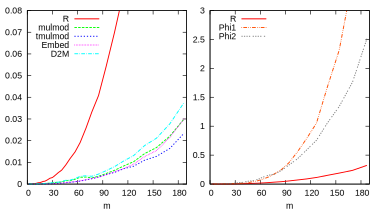
\includegraphics[width=0.5\textwidth]{creat}
  \caption{Timings in seconds, $p=5$, $n=m+1$}
  \label{fig:bench}
\vspace{-4ex}
\end{figure}

To demonstrate the practicality of our algorithms, we made a C
implementation and compared it to various ways of constructing the
same fields in Magma. All timings in this section are obtained on an
Intel Xeon E5620 CPU at 2.40GHz, using Magma V2.18-12, Flint 2.4.1 and
Sage 6.

Our implementation is limited to finite fields of word-sized
characteristic.  It is based on the C library
Flint~\cite{hart2010flint}, and we make it available as a Sage module
in an experimental fork at
\url{https://github.com/defeo/sage/tree/ff_compositum}. We plan to
make it available as a standard Sage module, as well as a separate C
library, when the code has stabilized.

Based on the observation that algorithms {\sf Embed} and {\sf Project}
are simpler than conversion algorithms between monomial and dual
bases, we chose to implement a \emph{lazy change of basis}
strategy. By this we mean that our Sage module (rather than the C
library itself) represents elements on either the monomial or the dual
basis, with one representation computed from the other only when
needed. For example, two elements of the same field can be summed if
both have a monomial or if both have a dual representation. Similarly,
two elements can be multiplied using standard multiplication if both
have a monomial representation, or using transposed multiplication if
one of the two has a monomial representation. In all other cases, the
required representation is computed and stored when the user input
prompts it. To implement this strategy efficiently, our Sage module is
written in the compiled language Cython.

We focus our benchmarks on the setting of Section \ref{sec:emb-iso}:
$P$ and $Q$ are two irreducible polynomials of coprime degrees $m$ and
$n$, and $R=P\odot Q$. We fix the base field $\F_p$ and make $m$ and
$n$ grow together with $n=m+1$. We measure the time to compute $R$, to
apply the algorithms {\sf Embed}, {\sf Phi1}, etc., and to compute the
changes of bases. We noticed no major difference between different
characteristics, so we chose $p=5$ for our demonstration. As shown in
Figure~\ref{fig:bench}, the dominating phase is the computation of $R$
(line labeled {\sf R}). Surprisingly, transposed modular
multiplication is slightly faster than ordinary modular
multiplication. The cost of {\sf Embed} is about the same as that of
multiplication, while {\sf DualToMonomial} is about 50\% slower. {\sf
  Project} and {\sf MonomialToDual} have, respectively, similar
performances (only slightly faster) hence they are not reported on the
graph. This justifies our design choice of \emph{lazy change of
  basis}.  

Unsurprisingly, the isomorphism algorithms take significantly more
time than the computation of $R$; for our choices of degrees, {\sf
  Phi2} is asymptotically faster than {\sf Phi1} and the crossover
between them happens around $m=70$. 

\begin{figure}
  \centering
  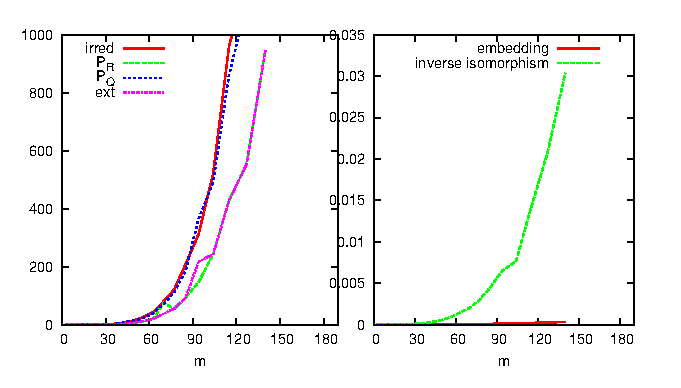
\includegraphics[width=0.5\textwidth]{magma}
  \caption{Magma timings in seconds, $p=5$, $n=m+1$}
  \label{fig:magma}
\vspace{-4ex}
\end{figure}

We compare our implementation to four different strategies available
in Magma. For each of them we measure the time to construct the finite
fields and embedding data, as well as the time to do operations
equivalent to {\sf Embed}, resp.\ inverse
isomorphism. Figure~\ref{fig:magma} reports on the following
experiments:
\begin{itemize}
\item In {\sf irred}, we supply directly $P$, $Q$ and $R$ to Magma's
  finite field constructor, then we call the \verb+Embed+ routine to
  compute the embedding data.
\item In  {\sf P R}, we use Magma's default constructor to compute $P$
  and $R$ (Magma chooses its own polynomials), then we call the
  \verb+Embed+ routine to compute the embedding.
\item In {\sf P Q}, we use Magma's default constructor to compute $P$
  and $Q$ (Magma chooses its own polynomials), then use the
  \verb+CommonOverfield+ routine to compute $R$, then \verb+Embed+ to
  compute the embedding data.
\item In {\sf ext}, we use Magma's default constructor to compute $P$,
  then the \verb+ext+ operator to compute an extension of degree $n$
  of $\F_p[x]/\ang{P}$ (Magma chooses its own polynomials).
\end{itemize}
Timings for constructing the extension and the embedding vary from one
method to the other; once this is done, timings for applying
embeddings or (inverse) isomorphisms are the same across these
methods.

The Magma implementation cannot construct the embedding data in large
cases ($m = 150$) in less than 1000 seconds, while our code takes a
few seconds. Once the embedding data is known, Magma can apply the
embeddings or isomorphisms extremely fast; in our case, one may do the
same, using our algorithms to compute the matrices of $\Phi$ and
$\Phi^{-1}$, when precomputation time and memory are not a concern.



\scriptsize
\bibliographystyle{plain} \bibliography{defeo}

\end{document}




% Local Variables:
% mode:flyspell
% ispell-local-dictionary:"american"
% mode:TeX-PDF
% mode:reftex
% End:

% LocalWords:  embeddings bilinear
